\documentclass[a4paper,12pt]{report}
\renewcommand\thesection{\arabic{section}}
\usepackage{helvet}
\renewcommand{\familydefault}{\sfdefault}
\renewcommand{\baselinestretch}{1.5} 
\usepackage{graphicx}
\usepackage{hyperref}
\graphicspath{ {images/} }
\begin{document}

\begin{titlepage} % Suppresses headers and footers on the title page
	
	\centering % Centre everything on the title page
	
	\scshape % Use small caps for all text on the title page
	
	\vspace*{\baselineskip} % White space at the top of the page
	
	%------------------------------------------------
	%	Title
	%------------------------------------------------
	
	\rule{\textwidth}{1.6pt}\vspace*{-\baselineskip}\vspace*{2pt} % Thick horizontal rule
	\rule{\textwidth}{0.4pt} % Thin horizontal rule
	
	\vspace{0.75\baselineskip} % Whitespace above the title
	
	{\LARGE Consultant Tracker\\Coding Standards} % Title
	
	\vspace{0.75\baselineskip} % Whitespace below the title
	
	\rule{\textwidth}{0.4pt}\vspace*{-\baselineskip}\vspace{3.2pt} % Thin horizontal rule
	\rule{\textwidth}{1.6pt} % Thick horizontal rule
	
	\vspace{2\baselineskip} % Whitespace after the title block
	
	
	%------------------------------------------------
	%	Editor(s)
	%------------------------------------------------
	
	Edited By
	
	\vspace{0.5\baselineskip} % Whitespace before the editors
	
	{\scshape\Large Sibekezelo Mamba 16095414 \\ Johan de Waal 16155140 \\ Stephen Munro 16024479\\ Hulisani Mudimeli 16073364 \\ Ngonidzashe Mujuru 16285256  \\ Tatenda Mafunga 16094965\\} % Editor list
	
	\vspace{0.5\baselineskip} % Whitespace below the editor list
	
	\textit{University of Pretoria \\2018} % Editor affiliation
	
	\vfill % Whitespace between editor names and publisher logo
	
\end{titlepage}
\newpage
\tableofcontents
\newpage
%\pagenumbering{arabic}
\section{Github Repository}
\subsection{Folders} 
Folder naming uses \underline{UpperCamelCase} \\
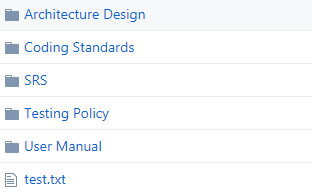
\includegraphics{Github}
\subsection{Files} 
File naming uses \underline{UpperCamelCase} \\
\includegraphics{fileNaming}

\section{Overview}
The following coding conventions pertain to how code is written and structured for the Consultant Tracking project. The standards are developed to be followed regardless of programming language used.

\section{File Names}
The preferred file naming style is \underline{UpperCamelCase} \\ \\
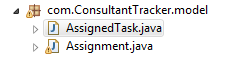
\includegraphics{Files}
\section{Formatting}
\subsection{Line Length} 
	- The maximum number of characters in a line should be 80.\\
	- Control structure conditions may exceed 80 characters, if they are simple to read and understand.\\
	- Statements containing queries that are clear may exceed 80 character:\\
	Example:\\ 
	
\includegraphics{Statement}  \\
	- Lines containing method/class names or variable declarations may exceed 80 characters.\\
	Example:\\ 
	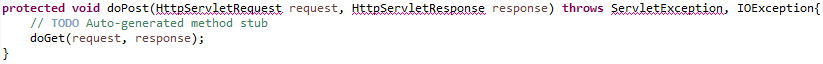
\includegraphics{LongMethodName}
\subsection{Line Wrapping}
	Conditions should not be wrapped in multiple lines, it is recommended to split the conditions.\\
	Do not use multiple statements on a single line if the length is going to exceed 80 characters.\\
	Introduce line break after the opening and closing braces.\\\\
	If a Line is too long because it contain a long expression, wrap using the following guides:\\
	1. Divide the expression into smaller subexpressions.\\
	2. Introduce a line break after each comma in the expression, and align each expression with the first character of the expression preceding the comma.\\
	3. Introduce a line break after the operator with the lowest precedence, until the line does not exceed the 80 character limit.
\subsection{Spacing}
One blank line should be used in the following cases:\\
\textbullet between methods\\
\textbullet Between the local variables in a method and its first statement.

\subsection{Use Of Parentheses}
Use parentheses on expressions containing mixed operators, do not assume other programmers understand precedence as well you as you do.
\subsection{Commenting}
Each class or function should contain at least one sentence that provide a description or summary of the entity.\\
Block comment may be used at the beginning of each file.\\
line comments must be followed by a newline, for easy readability.\\
Trailing comments must be shifted far enough to separate them from statements.\\
Commenting your code is great but avoid commenting obvious code.\\
Comments should not be long and overcomplicated. 

\section{Naming}
\subsection{Variable declaration}
Variable names are nouns and should provide a clear meaning of what the object is.
\subsection{Classes, Methods and Interface Declarations}
Class names are written in \underline{UpperCamelCase}.\\
Start Setter methods by \underline{set}, followed by Variable to set.\\
Start Getter methods by \underline{get}, followed by variable to get\\

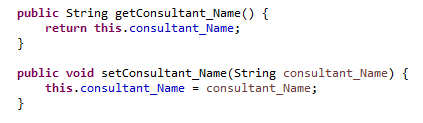
\includegraphics{MethodNames}

Class names uses \underline{UpperCamelCase}\\

\includegraphics{ClassName}
\section{Statements}
\subsection{Simple Statements}
Each line should contain at most one statement.
\subsection{Compound Statements}
Use Braces on all control statements inside the compound statement to reduce errors of forgetting to close braces.\\
Enclosed statements should be indented one more level than the compound statement for readability.  
\subsection{Return Statements}
If the return value is an expression use parentheses to provide clear meaning and precedence.
\subsection{If, If else Statements}
If statements should always use {}, avoid the error-prone form:\\ if(condition) statement //AVOID.\\
if(condition) \{ statement \} //USE. 
\subsection{For Statements}
for statement should have the following form:\\
for (initialization; condition; update) \{ \\
	\indent statements;\\
\} 
\subsection{While loop}
A while statement should have the following form:\\
while (condition) \{ \\
	\indent statements;\\
\}
\subsection{Do-While Loop}
A do-while statement should have the following form:\\
do \{ \\
	\indent statements; \\
\} while (condition); 
\subsection{try-catch Statements}
A try-catch statement should be in the following form, the finally block can be omitted. 
try \{ \\
	\indent statements;\\
\} catch (ExceptionClass e) \{ \\
	\indent statements;\\
\} finally \{
	\indent statements;\\
\}

\section{SAPUI5 Standards}
\subsection{Routing and navigation}
Navigation is implemented using manifest based routing.
\subsection{Developing views in application}
Use xml views in the project. Using different views will lead into problems while writing down the navigation logics.  
\subsection{Naming conventions}
	\subsubsection{Lists}
		Use camelCase:\\
		\indent listItem (Correct)\\
		\indent Listitem (Wrong)
	\subsubsection{Controller Names}
		Use camelCase:\\
		\indent	detailPageController (Correct)\\
		\indent	detail\_page\_controller (Wrong)
	\subsubsection{Parameter Names}
		Names should be descriptive and have maening. The name should give indication to the 		purpose of the paramater.\\
		\indent consultantId (Correct)\\
		\indent valueParameter (Wrong)


\subsubsection{Class Name}
		The naming should be first letter capital followed by camel casing for the remaining words.\\
		 \indent DetailConsultant, MasterConsultant  (Correct)\\
		\indent detail\_ consultant, detail-consultant, detailconsultant (Wrong)\\
		
\subsection{Comments}
		Comments should not rephrase the code, but tell the reader what is in the code. Describe why your code does what it does.  Line comments are preffered. Use block comments if more than 4 lines.


		

\section{Standards}
\subsection{Software Verification and Validation}
\subsection{Inspection}
The issue of code inspection was addressed by using Eclipse IDE. As the backend is done in Java, Eclipse was chosen as it is the most popular java IDE (White,2014) and it automatically checks common errors. The documentation was written by different members of the team and inspected by our Documentation Leader, Tatenda Mafunga.\\
\subsection{Walkthrough}
Manually executes the product using simple test data. Usually the developer who produces the product leads the team to perform the walkthrough. The team checks the product step by step while asking questions. A product walkthrough was carried out to ensure that the any inconsistencies would be ironed out. Stephen Munro, Backend team, led the walkthrough of the backend and the remainder of the team asked questions to clarify any misunderstandings and suggest improvements. Johan van De Waal led the walkthrough of the front-end, which was carried out in a similar fashion.\\
\subsection{Pair-Programming}
The integration of the front-end and the backend was carried out applying pair programming principles to ensure that the implementation was of a high quality. The code was done on one laptop with a member from the backend team and the front-end team taking the roles of driver and navigator. The members switched roles as often as they found necessary.

In carrying out the software verification and validation, the following agile principles were followed:   			
1. Good is good enough
2. Keep it simple and easy to do
3. Value working software over comprehensive documentation
\\
\subsection{References}

1.	White, O. 2014. IDEs vs. Build Tools: How Eclipse, IntelliJ IDEA \& NetBeans users work with Maven, Ant, SBT \& Gradle. Online Available at:
\url{https://zeroturnaround.com/rebellabs/ides-vs-build-tools-how-eclipse-intellij-idea-netbeans-users-work-with-maven-ant-sbt-gradle/#disqus_thread}
Accessed 05/05/18\\

\end{document}